\subsubsection{Frontend erstellen}
Zu dem Frontend des Produktes gehören alle Elemente, auf welche der Benutzer Einsicht hat und mit denen er interagieren kann. Diese sind besonders für die Benutzbarkeit des Produkt wichtig, da diese die wichtigste Produktqualität ist.

\paragraph{Aktivitätsdiagramm Frontend}\mbox{}\\
\begin{figure}[H]
	\centering
	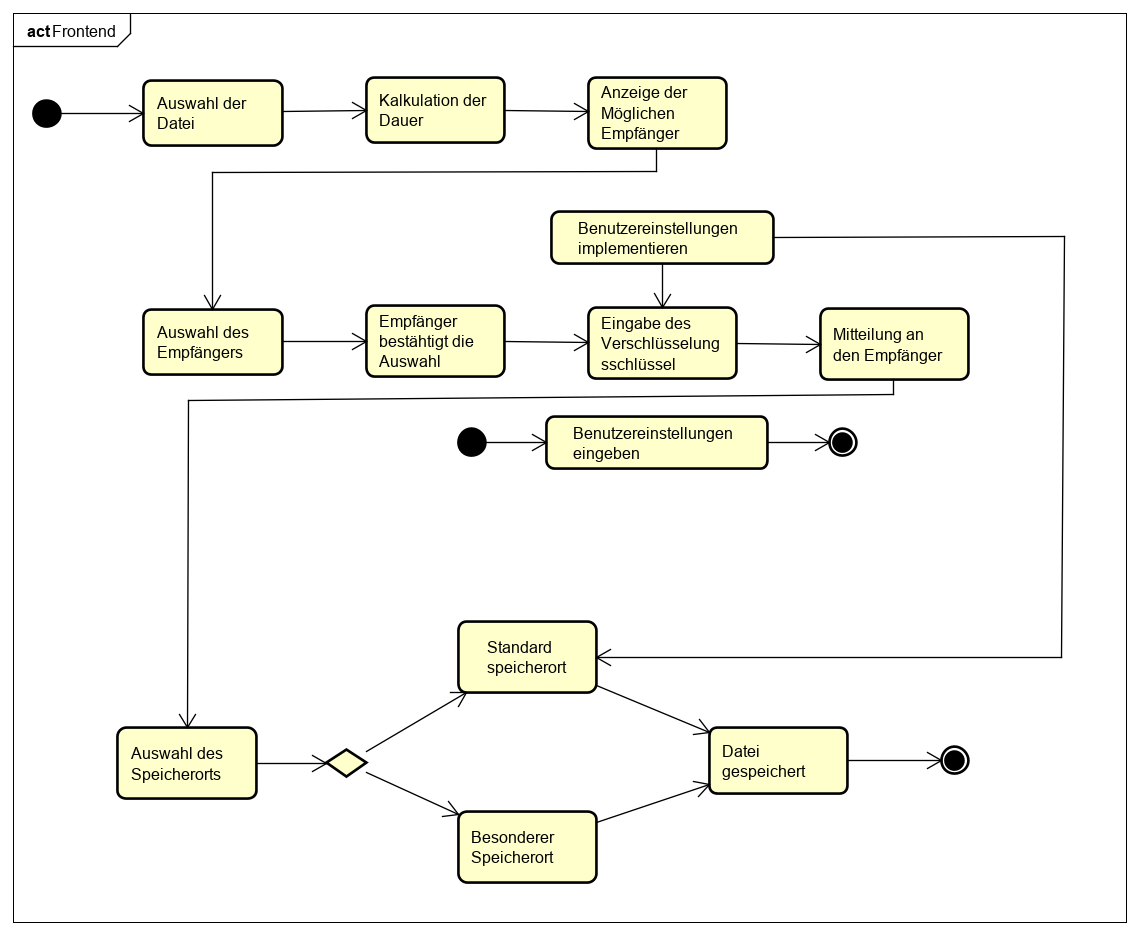
\includegraphics[width= 0.9\linewidth]{diagramms/activity/Frontend.png}
	\caption{Aktivitätsdiagramm Frontend}
\end{figure}
\newpage
\begin{indentE}\mbox{}
	\paragraph{/LF2210/ Datei auswählen}\mbox{}\\
	Der Benutzer wählt eine Datei aus, welche er verschicken möchte. Hierbei soll eine voreilige Kalkulation durchgeführt werden, welche die Dauer der Übertragung schätzt.
	\UseCase{
		{App Frontend}
		{/LF2210/ Datei auswählen}
		{Frontend}
		{Ein wird die zu versendende Datei ausgewählt.}
		{Es muss die Datei, welche versendet werden soll, ausgewählt werden}
		{Es kann die Datei gesendet werden}
		{Sender}
		{Datei(Name, Größe, Inhalt)}
		{Es kann keine Datei ausgewählt werden}
		{Es kann eine zu versendende Datei ausgewählt werden}
		{hoch}
		{mittel}
		{Should Have}
	}
	\paragraph{/LF2220/ Empfänger auswählen}\mbox{}\\
	Es werden dem Benutzer die möglichen Empfänger angezeigt und ausgwählt oder er kann den Namen des Empfängers eingeben, um den Empfänger zu bestimmen. Dieser muss die Verbindung bestätigen.
	\UseCase{
		{App Frontend}
		{/LF2220/ Empfänger auswählen}
		{Frontend}
		{Der Sender wählt anhand des Namens den Empfänger aus, mit dem der Datentransfer stattfinden soll.}
		{Es muss der Empfänger ausgewählt werden.}
		{Die Verbindung kann aufgebaut werden}
		{Sender, Empfänger}
		{Sendername, Empfängername}
		{Es kann kein Empfänger ausgewählt werden.}
		{Es kann anhand des Namens der Empfänger der Datei ausgewählt werden.}
		{hoch}
		{mittel}
		{Should Have}
	}
	\paragraph{/LF2230/ Verschlüsselungsschlüssel eingeben}\mbox{}\\
	Wenn kein Standard-Schlüssel ausgewählt ist, muss der Sender diesen bevor dem Verbindungsaufbau eingeben. Dieser muss dann dem Empfänger mitgeteilt werden und dieser muss den selben auch eingeben, um den Datentransfer zu ermöglichen.
	\UseCase{
		{App Frontend}
		{/LF2230/ Verschlüsselungsschlüssel eingeben}
		{Frontend}
		{Es müssen Empfänger und Sender einen Schlüssel eingeben, die übereinstimmen, um den Datentransfer zu beginnen.}
		{Der Datentransfer muss mit einem Schlüssel verschlüsselt werden.}
		{Der Datentransfer kann verschlüsselt werden}
		{Sender, Empfänger}
		{Schlüssel}
		{Die Daten können nicht mit einem Schlüssel verschlüsselt werden}
		{Die Daten können mit einem frei wählbaren Schlüssel verschlüsselt werden}
		{hoch}
		{mittel}
		{Should Have}
	}
	\paragraph{/LF2240/ Datei speichern}\mbox{}\\
	Der Empfänger soll nach dem empfangen der Datei auswählen können, ob diese im Standard-Speicherort gespeichert wird, oder in einem besonderen. Wenn der Besondere ausgewählt worden ist, soll ihm ein Benutzerinterface gezeigt werden, indem er den Speicherort auswählen.
	\UseCase{
		{App Frontend}
		{/LF2240/ Datei speichern}
		{Frontend}
		{Der Empfänger soll den Speicherort des bekommenen Datei auswählen können.}
		{Die Datei muss irgendwo gespeichert werden}
		{Der Speicherort der Datei kann ausgewählt werden}
		{Empfänger}
		{Datei(Name, Größe, Inhalt), Speicherort}
		{Die Datei wird entweder immer am selben Ort, oder nicht gespeichert}
		{Der Speicherort kann frei gewählt werden}
		{mittel}
		{gering}
		{Should Have}
	}
	\paragraph{/LF2250/ Benutzereinstellungen hinzufügen}\mbox{}\\
	Der Benutzer kann einige Fix-Einstellungen auf seinem Produkt tätigen. Darunter zählt die Möglichkeit, den Namen zu ändern, welcher den restlichen Nutzern angezeigt wird, die Verschlüsselung zu aktivieren oder deaktivieren, einen Standardschlüssel auszuwählen und einen Standard-Speicherort auszuwählen. Dabei sollen die eingegebenen Daten auf ihre Korrektheit überprüft werden.
	\UseCase{
		{App Frontend}
		{/LF2250/ Benutzereinstellungen hinzufügen}
		{Frontend}
		{Der Benutzer kann verschiedenen Einstellungen tätigen, mit welche er die Datenübertragung beeinflussen kann.}
		{Die Einstellungen müssen auf einem Interface getätigt werden}
		{Die Einstellungen können getätigt werden}
		{Empfänger, Sender}
		{gewünschter Systemname, Verschlüsselung(Ja/Nein), Standardschlüssel, Standard-Speicherort}
		{Das Produkt kann nicht angepasst werden.}
		{Es können Einstellungen getroffen werden, welche das Produkt beeinflussen.}
		{mittel}
		{mittel}
		{Nice to Have}
	}
	\paragraph{/LF2260/ Appinterface designen}\mbox{}\\
	Es muss ein Interface für das Smartphone entworfen werden. Dazu gehören Mockups und Prototypen. Diese müssen vor deren Implementierung vom Auftraggeber bestätigt werden.
	\UseCase{
		{App Frontend}
		{/LF2260/ Appinterface designen}
		{Frontend}
		{Es müssen Mockups für die Appinterfaces erstellt werden. Diese diene als Vorlage für die Interfaces.}
		{Für einen schnellere und besser Implementierung sollen Mockups als Vorlage dienen.}
		{Die Implementierung ist einfacher, schneller und besser.}
		{Auftraggeber, Auftragnehmer}
		{}
		{Das Interface wird ohne Vorlage erstellt.}
		{Das Interface kann nach einer vom Auftraggeber bestätigten Vorlage erstellt werden.}
		{mittel}
		{gering}
		{Nice to Have}
	}
	\paragraph{/LF2270/ Appinterface implementieren}\mbox{}\\
	Das Appinterface muss nach der Bestätigung des Auftraggeber implementiert werden. 
	\UseCase{
		{App Frontend}
		{/LF2270/ Appinterface implementieren}
		{Frontend}
		{Das Appinterface muss durch die Mockups realisiert werden.}
		{Der Benutzer hat keine Möglichkeit mit dem System zu integrieren}
		{Der Benutzer kann mit dem System interagieren und dadurch dessen Funktionen benutzen.}
		{Benutzer}
		{sämtliche Nutzereingaben}
		{Der Benutzer kann mit dem System nicht interagieren}
		{Der Benutzer ist in der Lage mit dem System zu interagieren}
		{hoch}
		{hoch}
		{Should Have}
	}
	\paragraph{/LF2280/ Frontend und Backend verbinden}\mbox{}\\
	Es muss eine Verbindung zwischen dem Frontend und Backend erstellt werden, welche die Aufforderungen verarbeitet und zum Backend weiterleitet. Diese Verbindung, soll dem Benutzer entweder mitteilen, wie lange die Verarbeitung noch dauert oder bei kürzeren das wiederholte Aufrufen von Aufforderungen verhindern.
	\UseCase{
		{App Frontend}
		{/LF2280/ Frontend und Backend verbinden}
		{Frontend}
		{Das Frontend muss mit dem Backend verbunden werden, um die Nutzereingaben an das Backend weiterzuleiten. Außerdem soll es Daten ans Frontend schicken, welche über momentane Prozess aufklärt.}
		{Die Daten müssen vom Frontend ans Backend und umgekehrt geschickt werden}
		{Das Frontend kann mit dem Backend und umgekehrt kommunizieren.}
		{Benutzer}
		{sämtliche Nutzereingaben und verwertete Daten}
		{Die Nutzerdaten können nicht an das Backend und die verwerteten Daten nicht ans Frontend geschickt werden.}
		{Daten können zwischen Frontend und Backend ausgetauscht werden.}
		{hoch}
		{mittel}
		{Should Have}
	}
\end{indentE}